%!TEX encoding = UTF-8 Unicode
\subsection{Fog computing architecture}
Fog computing is a great resource to support IoT applications' requirements. Taking into account what has been mentioned in Section \ref{sec:Introduction} and Section \ref{sec:Computingparadigms}, fog computing has, the below, eight fundamental characteristics which validate the statement uttered above \cite{iorga2018fog}:
\begin{itemize}
	\item \textbf{Contextual location awareness, and low latency}. Provides low latency due to the proximity between the IoT devices and the fog nodes. Also, the contextual location allows them to be aware of the cost of communication latency with both other fog nodes and the end devices, allowing the distribution of applications across the network to be organized in a weighted manner;
	\item \textbf{Geographical distribution}. Uses anything between the cloud and \textit{things} to provide ubiquitous computing, allowing continuity of service in mobile environments;
	\item \textbf{Heterogeneity}. Supports wide diversity of communications, applications and services;
	\item \textbf{Interoperability and federation}. Uses cooperation of different providers to support heavy applications such as real-time streaming. Moreover, it supports migration of applications to more suited fog servers depending on the current context;
	\item \textbf{Real-time interactions}. Applications may involve real-time interactions rather than batch processing (e.g., as cloud does);
	\item \textbf{Scalability and agility of federated, fog-node clusters}. Fog is adaptive; may form clusters-of-nodes or cluster-of-clusters to support elastic compute, resource pooling, etc;
	\item \textbf{Predominance of wireless access}. Most of the end devices only support wireless communication;
	\item \textbf{Support for mobility}. The exponential growth of mobile devices demands mobility support.
\end{itemize}

Nonetheless, fog still has some limitations (as stated in Section \ref{subsec:Objectives}). In order to tackle those limitations, first it is needed an overview over its architecture. This includes understanding what are the actors and how they interact, how IoT nodes connect to the fog servers, how clients outsource the allocation and management of resources that they rely upon to these servers, how the location-aware and migration features are performed, etc.

\subsubsection{Overview}
\noindent\tab Fog computing is composed by fog nodes/servers, that allow the deployment of distributed, latency-aware applications and services. Those nodes can be either virtual (e.g., gateways, switches, routers, servers) or physical (e.g., virtualized switches, virtual machines, cloudlets) components that provide computing resources to end devices. They can be organized in clusters either vertically (to support isolation), horizontally (to support federation), or relative to fog nodes’ latency-distance to the IoT devices \cite{iorga2018fog}. Fog nodes can be accessed through connected devices located at the edge, which provide local computing resources and, when needed, provide network connectivity to centralized services (i.e. cloud). Moreover, fog nodes can operate in a centralized or decentralized manner and can be configured as stand-alone nodes.\\
\noindent\tab Fig. \ref{fog_architecture} shows the typical fog computing architecture. As stated before, mist computing can be implemented in a layer between the fog servers and the end devices. Moreover, the presence of cloud servers is not imperative, however it is very important for numerous applications.
\begin{figure} [t]
	\centering
	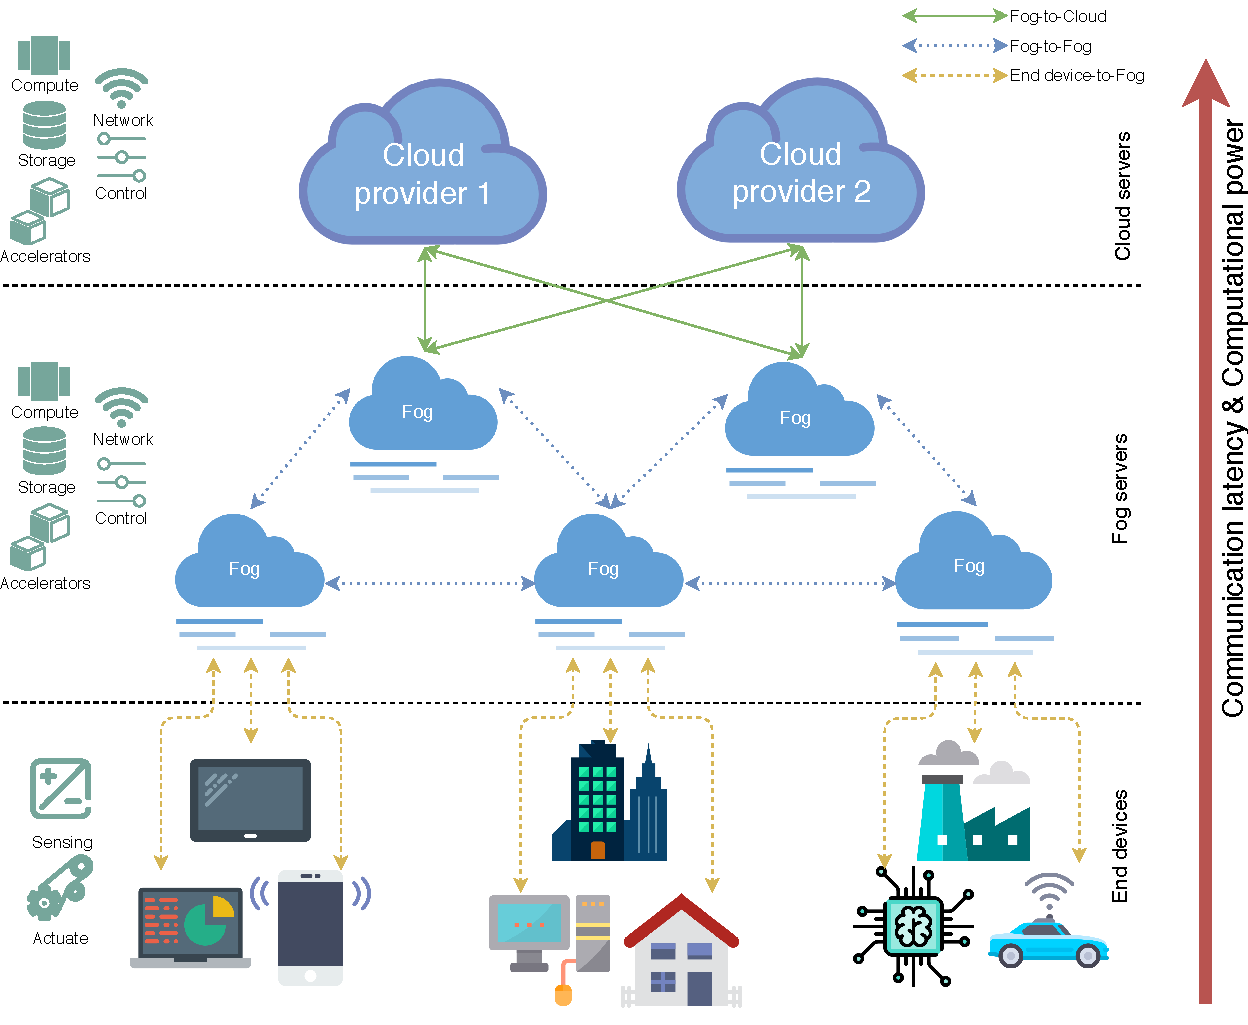
\includegraphics[width=0.9\textwidth]{images/fog_architecture/fog_architecture}
	\caption{Typical architecture of fog computing.}
	\label{fog_architecture}
\end{figure}
It is worth noting that, once fog nodes can be anything with computational and storage power in the cloud-to-things continuum, the links formed in these architectures (i.e. End device-to-Fog, Fog-to-Fog and Fog-to-Cloud) can be of any type. For instance, end devices can be connected to fog servers by wireless access technologies (e.g., WLAN, WiFi, 3G, 4G, ZigBee, Bluetooth) or wired connection. Moreover, fog nodes can be interconnected by wired or wireless communication technologies and they can be linked into the cloud by IP core network. Nonetheless, in order to provide location awareness, the fog layer also needs Location-Based Services (LBSs) that provide location information.

\noindent\tab In this architecture, the connected sensors located at the edge, generate data that can adopt two models. First, in a sense-process-actuate model, the information collected is transmitted as data streams, which is acted upon by applications running on fog devices and the resultant commands are sent to actuators. In this model, the raw data collected often does not need to be transferred to the cloud; data can be processed, filtered, or aggregated in fog nodes, producing reduced data sets. The result can then be stored inside fog nodes or actuated upon through the actuators. Second, in a stream-processing model, sensors send equally data streams, where the information mined (from the incoming streams) is stored in data centers for large-scale and long-term analytics. In this case, big data needs to be stored and does not have that much latency constraints. Being fog servers less powerful than the cloud ones, cloud is far more suited for this kind of operations. Yet, fog servers can still shrink data, doing some intermediate processing as in the previous model. This meets the aforementioned statement - although cloud is not essential for the functioning of fog, in some applications it is beneficial or even essential.\\
\noindent\tab Fog servers are the fundamental components in this three tier architecture (i.e. IoT-fog-cloud). They are able to support the six features shown below \cite{iorga2018fog}:
\begin{itemize}
	\item \textbf{Autonomy}. Fog nodes can be autonomous enough to operate independently, making local decisions, at the node or cluster-of-nodes level;
	\item \textbf{Heterogeneity}. Can be deployed in a wide variety of environments;
	\item \textbf{Hierarchical clustering}. The fog network can be organized with different numbers of layers, so that they are able to provide different subsets of service functions while working together as a continuum;
	\item \textbf{Manageability}. They are managed and orchestrated by complex systems that can perform most routine operations automatically;
	\item \textbf{Programmability}. Fog nodes are inherently programmable at multiple levels, by multiple stakeholders such as network operators, domain experts, equipment providers, or end users.
\end{itemize}
\noindent\tab Fog nodes generally are of most value in scenarios where data needs to be collected at the edge and where the data from thousands or even millions of devices is analyzed and acted upon in micro and milliseconds \cite{openfog2017openfog}. In order to being able to support such a large number of requests, especially those engaged in enhanced analytics, fog nodes may implement additional hardware. Accelerators modules (refer to Fig. \ref{fog_architecture}) can be implemented to provide supplementary computational throughput. For instance, hardware accelerators can be performed through Graphics Processing Unit (GPUs); they are an optimal choice for applications that support parallelism or for stream processing. Also, fog nodes can opt to make use of Field Programmable Gate Arrays (FPGAs) or even Digital Signal Processors (DSPs) for this propose.

\subsubsection{Data Placement}
\noindent\tab The applications deployed by the end users in fog nodes can be seen either as a whole or as a Distributed Data Flow (DDF) model, in which the applications are moduled as a collection of modules. This can be particular useful so that the less restricted modules in terms of latency can be deployed to the upper fog layers (ideally to the cloud), leaving the fog nodes of the lower layers less overloaded, being able to respond faster to modules within tighter latency bounds. Nonetheless, fog nodes can communicate between them to perform data and process management in order to support application requirements, as well as to exchange fog control/management data such as user device and application state.\\






\cite{giang2015developing}
This paper proposes a Distributed Dataflow (DDF) programming model for the IoT that utilizes computing infrastructures across the Fog and the Cloud. Also, evaluate their proposal by implementing a DDF framework based on Node-RED (Distributed Node-RED or D-NR), a visual programming tool that uses a flow-based model for building IoT applications. To address challenges of the intrinsic nature of the IoT (heterogeneous devices/resources, a tightly coupled perception-action cycle and widely distributed devices and processing), they propose a Distributed Dataflow (DDF) programming model for the IoT that utilities computing infrastructures across the Fog and the Cloud. Also, they evaluate their proposal by implementing a DDF framework based on Node-RED (Distributed Node-RED or D-NR), a visual programming tool that uses a flow-based model for building IoT applications.\\

\cite{bahreini2017efficient}
The authors address the problem of multi-component application placement on fog nodes. Each application could be modeled as a graph, where each node is a component of the application, and the edges indicate the communication between them.\\

\subsubsection{Virtualization Mechanisms}
In general, hosting an application involves creating a set of virtual machines (VMs) or execution containers (e.g., Docker) and assigning them a vector of computing resources (such as CPU, memory and storage) from the physical machines (PMs) in the edge-cloud.

%ver \cite{saurez2016incremental} & iCanCloud

\cite{li2018virtual}
They propose a layered Fog framework to better support IoT applications through virtualization. The virtualization is divided into object virtualization  (VOs), network function virtualization and service virtualization. VOs to address the protocol inconsistency (lack of unified networking protocols that leads to exaggerated overhead); Network function virtualization maps standard networking services to VOs, thus, minimize the communication process between consumers and producers by minimizing latency, improving security and scalability; Service virtualization that composes the community and Cloud Apps from various vendors to serve local Fog users with high quality of experience (QoE) but at low cost. At last, Foglets are involved to seamless aggregate multiple independent virtual instances, Fog network infrastructures, and software platforms.\\

\cite{bruschi2018move}
With the state-of-the-art virtualization technologies, services can be implemented in modular software as a graph/chain of portable VOs that can be dynamically migrated around the Telco infrastructure. It is proposed a VO clustering and migration policy that jointly considers user proximity and inter-VO affinity to scalably support user mobility, while allowing service differentiation among users.\\

\subsubsection{Orchestration}
\noindent\tab When an end device needs to offload some work to a third party, it needs somehow to know where to outsource the allocation and management of resources that they rely upon. For this propose, the fog architecture also needs a discovery and orchestration service which concerns in finding the best available fog server, given certain capabilities and requirements.\\

\noindent\tab In this context, E Saurez et al. \cite{saurez2016incremental} propose foglets, a programming model that facilitates distributed programming across fog nodes. Foglets are implemented in fog nodes using container technology. They provide APIs for app development as a dataflow graph whose nodes can be placed in the different levels of the computational hierarchy. In additional to the provided primitives for communication between the application components, it also embodies algorithms for the discovery and incremental deployment of resources commensurate with the application needs. Moreover it provides mechanisms for QoS-sensitive and workload sensitive migration of application components due to end devices mobility and application dynamism. Specifically they show that there are four entities in the foglets runtime system: the discovery server, the docker registry server, the entry point daemon, and finally the worker process. The discovery server is a partitioned name server that maintains a list of fog nodes available. Docker registry server is a server that contains the binaries for the applications that have been launched on the foglets infrastructure. The entry point daemon executes directly on top of the host OS in the fog node, awaits requests and periodically sends ``I am alive'' message to the discovery server. Finally the worker process that will carry out the functionality contained in a particular application component assigned to it.\\

\noindent\tab Also in this context, F Bonomi et al. \cite{bonomi2014fog} propose a fog computing layer architecture that is classified into two sub-layers: (1) the fog abstraction layer, and (2) the fog orchestration layer. While the former enables virtualization, provides data and resource isolation guarantees, manages the fog resources, and preserves security and privacy, the latter provides dynamic, policy-based life-cycle management of fog services. The fog orchestration layer comprises of a software agent, Foglet, with reasonably small footprint yet capable of bearing the orchestration functionality and performance requirements. Moreover, this layer also needs a distributed, persistent storage to store policies and resource meta-data (e.g., capability, performance) that support high transaction rate update and retrieval, a scalable messaging bus to carry control messages for service orchestration and resource management and finally a distributed policy engine with a single global view and local enforcement.\\

\noindent\tab Julien Gedeon \cite{gedeon2017router}, propose a brokering mechanism in which available surrogates (e.g., cloudlets) advertise themselves to the broker. The broker receives client requests and considers a number of attributes such as network information, hardware capabilities, and distance to find the best available surrogate for the client. They look at the problem of surrogate discovery in the context of an urban area, where they are faced with a high mobility of end devices. Multiple brokers are interconnected using Distributed Hash Tables (DHTs) in order to exchange information.\\

\subsubsection{Concluding Remarks}
%Applications that require characteristics such as low latency, geo-distribution, mobility, high resilience, and large-scale distributed systems benefit from the Fog.
\noindent\tab Fog servers can provide reduced latencies and help in avoiding/reducing traffic congestion in the network core. However, this comes at a price: more complex and sophisticated resource management mechanisms are needed. This raises new challenges to be overcome such as dynamically deciding when, and where (device/fog/cloud) to carry out processing of requests to meet their QoS requirements. Furthermore, in mobile environments such mechanisms must incorporate mobility (i.e. location) of data sources, sinks and fog servers in the resource management and allocation process policies to promote and take advantage of proximity between fog and users.